\documentclass[Interploate_hadwritten_Digits.tex]{subfiles}

\begin{document}
	\subsection{Aufbereitung der Daten}
	Als Datensatz wurde der MNIST Datensatz von der offiziellen Webseite\footnote{\cite{lecun-mnist}} von Yann LeCun verwendet. Dieser umfasst ein Trainingsset von \numprint{60000} und ein Testset von \numprint{10000} klassifizierten Bildern mit handgeschriebenen Ziffern. Diese sind in zwei verschiedenen Dateien aufgeteilt, eine für die Bilder und eine für die Labels. Von der Bilder-Datei werden jeweils 28x28 Bytes eingelesen, welche ein Bild repräsentieren und in einen 784-dimensionalen Vektor geschrieben. Dabei werden die 255 Graustufenwerte auf Gleitkommazahlen zwischen Null und Eins verwandelt. Die Label-Datei wird Byteweise eingelesen und in eine One-Hot Vektor der Länge zehn verwandelt, bei welchem der Index der Eins dem Wert des Labels entspricht.
	
	\subsection{Das Modell erstellen und trainieren}
	Das Neuronale Netz wurde mit Tensorflow\footnote{\cite{tensorflow}} modelliert und trainiert. Das verwendete Modell ist ein Feed Forward Neuronal Network mit Weights und Biases für jede Schicht. Um den Output des Netzes zu berechnen, muss $ \vec{x_{n}} $ berechnet werden. Dabei is $ \vec{x_{0}} $ der Bildvektor. Die restlichen Werte werden gemäss Gleichung \ref{eq:layer_calculation} berechnet. $ n $ entspricht dabei der Anzahl Schichten im Neuronalen Netz.
	\begin{equation}
	\vec{x_{i}} = a(\vec{x_{i-1}} \times w_{i-1} + b_{i-1})
	\label{eq:layer_calculation}
	\end{equation}
	
	Als Aktivierungsfunktion $ a(x) $ wird die Logistische Sigmoidfunktion verwendet, welche der Gleichung \ref{eq:sigmoid} zu entnehmen ist. Sie wird auf alle Elemente im Vektor $ \vec{x} $ angewendet. 
	\begin{equation}
	a(x)=\frac{1}{1+e^{-x}}
	\label{eq:sigmoid}
	\end{equation}
	Sie hat die Aufgabe zu verhindern, dass Zahlen durch die Matrixmultiplikationen zu gross im positiven oder negativen Raum werden. Dies erreicht die Funktion in dem sie den Definitionsbereich von $ [-\infty, \infty] $ auf den Wertebereich $ [0, 1] $ einschränkt. Dieses Verhalten wurde in der Abbildung \ref{fig:sigmoid_plot} visualisiert. So ist die Eingabe für jede Schicht im Netzwerk ein Vektor mit Werten zwischen Null und Eins, welcher der Stärke der Aktivierung jedes Neurons in dieser Schicht entspricht.
	\begin{Figure}
		\centering
		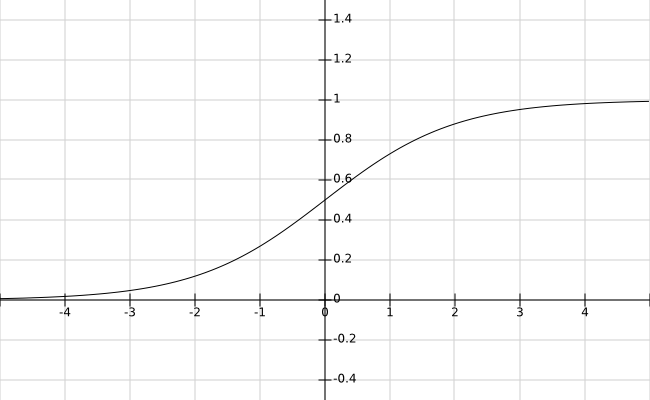
\includegraphics[width=\linewidth]{img/sigmoid_plot.png}
		\captionof{figure}{Verhalten der Sigmoid Funktion}
		\label{fig:sigmoid_plot}
	\end{Figure}

	Um das Neuronale Netzwerk zu trainieren muss der Fehler der Klassifikation berechnet werden. Dieser wird mit der Kreuzentropie zwischen dem normalisierten Output-Vektor $ \vec{x} $ des Netzwerks und dem Label-Vektor $ \vec{y} $ berechnet. Die Formel für die Kreuzentropie ist in Gleichung \ref{eq:cross_entropy} zu sehen.
	\begin{equation}
	H(\vec{x}, \vec{y}) = -\sum_{n}^{k}x_{k}log(y_{i})
	\label{eq:cross_entropy}
	\end{equation}
	Die Normalisierung des Vektors wurde mit der Softmax-Funktion aus der Gleichung \ref{eq:softmax}  realisiert. Dies hat zur Folge, dass alle Werte des Vektors im Bereich $ [0, 1] $ liegen und die Länge des Vektors eins beträgt. Durch diese Eigenschaften kann der Vektor als diskrete Wahrscheinlichkeitsverteilung für das Erkennen der Ziffer im Input-Vektor betrachtet werden.
	\begin{equation}
	\sigma(v)_{i} = \frac{e^{v_{i}}}{\sum_{n}^{k=1}e^{v_{k}}}
	\label{eq:softmax}
	\end{equation}
	
	Für die Korrektur des Fehlers im Neuronalen Netz wird ein Gradientenverfahren eingesetzt, welches den über die Kreuzentropie berechneten Fehler minimiert. In diesem Verfahren wird die Ableitung des Modells bestimmt und jeder Parameter um einen bestimmten Betrag in die Richtung des steilsten Abfalls korrigiert. In diesem Modell sind die Weight-Matrizen und Bias-Vektoren die Parameter. Der Korrekturbetrag ergibt sich aus der Steigung am Punkt der Funktion und dem Hyperparameter der Learning Rate.
	\begin{equation}
	b = a - \gamma \Delta f(a)
	\label{eq:gradient_decent}
	\end{equation}
	Das grundlegende Konzept des Gradientenverfahrens kann der Gleichung \ref{eq:gradient_decent} entnommen werden. Der neue Wert des Parameters $ b $ ergibt sich aus dem Lerning Rate $ \gamma $ multipliziert mit der Richtung des steilsten Abfalls $ \Delta f(a) $ subtrahiert vom ursprünglichen Wert $ a $. Dieses Verfahren wurde in der Abbildung \ref{fig:gradient_decent} visualisiert.
	\begin{Figure}
		\centering
		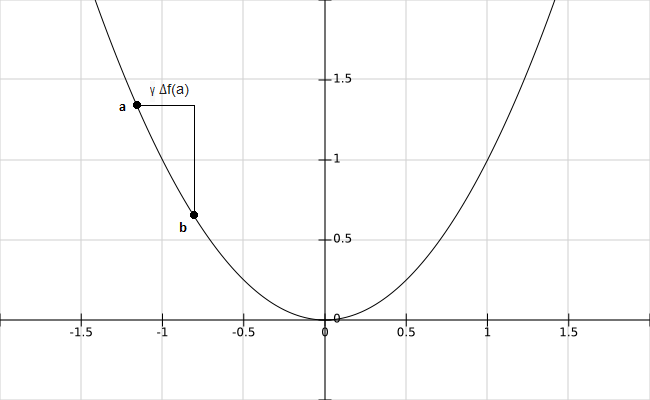
\includegraphics[width=\linewidth]{img/gradient_decent.png}
		\captionof{figure}{Visualisierug Gradientenverfahren}
		\label{fig:gradient_decent}
	\end{Figure}
	
	\subsection{Invertierung des Neuronalen Netzes}
	\label{sec:method_compress}
	Um die Funktion des Neuronalen Netzes zu invertieren wurde in einem ersten Schritt eine komprimierte Version des Netzes erstellt. Diese Komprimierung bestand darin die Weight-Matrizen und Bias-Vektoren in den homogenen Raum zu transformieren. Dadurch kann die Addition des Bias-Vektors und die Multiplikation der Weight-Matrix wie in Gleichung \ref{eq:homogenize_layer} beschrieben in eine Matrix pro Layer zusammengefasst werden. 
	\begin{equation}
		M_{i} =
		\begin{bmatrix}
		I & \vec{b_{i}} \\ 
		\vec{0}^{T} & 1
		\end{bmatrix}
		\times
		\begin{bmatrix}
		w_{i} & \vec{0} \\ 
		\vec{0}^{T} & 1 
		\end{bmatrix}
		\label{eq:homogenize_layer}
	\end{equation}
	
	Als nächster Schritt wurde versucht die Matrizen aller Layers in eine Matrix zusammenzuführen. Diese könnte später mit dem Inputvektor multipliziert werden und so alle Schritte im Neuronalen Netz auf eine Matrixmultiplikation reduzieren. Dies wurde gemäss der Gleichung \ref{eq:network_compression} gemacht. Dabei wurde angenommen, dass die Aktivierungsfunktion auf das Produkt der Matrixmultiplikation angewendet werden könnte, da deren Funktion das Einschränken des Wertebereichs ist. Diese Annahme erwies sich jedoch als falsch, was im Kapitel \ref{sec:results_compression} aufgegriffen wird. Aus diesem Grund wurde eine zweite Methode verwendet, bei welcher die Aktivierungsfunktion in der Komprimierung weggelassen wurde und nur auf das Resultat der Matrixmultiplikation mit dem Inputvektor angewendet.  Auch diese Methode ergab keine gültige Komprimierung.
	\begin{equation}
		N_{0} = M_{0},
		N_{i} = a(M_{i} \times N_{i - 1})
		\label{eq:network_compression}
	\end{equation}
	
	Da die Komprimierung des gesamten Netzes scheiterte, wurde nur die Komprimierung der einzelnen Layers beibehalten. Um das Netz zu invertieren wurde das Inverse aller Layer-Matrizen $ M_{i} $ berechnet. Da nicht alle Matrizen mit beliebigen Dimensionen eine echtes Inverse besitzen, wird die inverse Matrix mit Pseudoinverse approximiert. Gemäss der Dokumentation der verwendeten Library\footnote{\cite{numpy}} wird dies über die KQ-Methode erreicht. Das Inverse des Neuronalen Netzes ist so durch die Gleichung \ref{eq:feed_backwards} gegeben.
	\begin{equation}
		\vec{x_{i}} = a(M_{i-1}^{+} \times \vec{x_{i-1}})^{-1}
		\label{eq:feed_backwards}
	\end{equation}
	Dabei ist $ a(x)^{-1} $ das Inverse der Aktiverungsfunktion und definiert durch die Gleichung \ref{eq:sigmoid_inverse}.
	\begin{equation}
		a(x)^{-1} = -log_{e}(\frac{1}{x} - 1)
		\label{eq:sigmoid_inverse}
	\end{equation}
	
	Da das Pseudoinverse nicht garantiert ein echtes Invers ist, könnte dies einen Einfluss auf die berechneten Bilder haben. Aus diesem Grund wurde ein weiteres Neuronales Netz trainiert, welches sich desselben Modells bedient, jedoch die nur quadratische Matrizen verwendet. So konnte sichergestellt werden, dass alle Matrizen $ M_{i} $ im komprimierten Netz ein echtes Invers haben.
	
	\subsection{Approximation von Input Bildern}
	Bei der Evaluation des invertieren Neuronalen Netzes konnte eine mögliche Fehlerquelle für verfälschte Resultate ausfindig gemacht werden: Gleitkommazahlen verursachen in Computer Rundungsfehler. Diese sind in der Regel insignifikant, werden aber durch die inverse Sigmoidfunktion verstärkt und in einen signifikanten Bereich gebracht. Wie stark sich diese Rundungsfehler auf die Resultate auswirkt wurde im Rahmen dieser Arbeit ebenfalls untersucht und die Resultate sind im Kapitel \ref{sec:results_error_inverse} einzusehen.
	
	Um diese Fehlerquelle zu umgehen wurde ein weiteres Neuronales Netz trainiert. Dieses Neuronale Netz verwendet das gleiche Modell wie das ursprüngliche Netz. Der Unterscheid besteht darin, dass die Weigth-Matrizen und Bias-Vektoren als Konstanten definiert und als variabler Teil für die Optimierung der Input gewählt wurde. In diesem Modell versucht das Gradientenverfahren ein zufälliges Inputbild so zu verändern, dass dieses möglichst genau dem gesuchten Vektor im Zielraum entspricht.
\end{document}